\documentclass[a4paper]{article}

\usepackage{ablpreamble}
\usepackage{physics}
\AtBeginDocument{\RenewCommandCopy\qty\SI}
\ExplSyntaxOn
\msg_redirect_name:nnn { siunitx } { physics-pkg } { none }
\ExplSyntaxOff

\newtheorem{theorem}{Theorem}[section]
\newtheorem{corollary}{Corollary}[theorem]
\newtheorem{lemma}[theorem]{Lemma}

\theoremstyle{definition}
\newtheorem{definition}{Def}
\newtheorem{example}{Example}[section]

\title{Combinatorics}
\author{}

\begin{document}

\maketitle

\begin{definition}[Alphabet]
  ,,Set'' of objects. \(A\), \(X\), \(\Sigma\)
\end{definition}

\begin{definition}
  \[[n] = \{1, 2, \ldots n\}\]
\end{definition}

\section{Ordered arrangements}

\begin{definition}[Ordered arrangements]
  An ordered arrangement of \(n\) elements from alphabet \(\Sigma\) is a map
  \(s : [n] \to \Sigma\)
\end{definition}

Range of a function:
\[\ran s = \{ s(i) \mid i \in [n] \}\]

\begin{definition}[\(\Sigma\)-string]
 \(\Sigma\)-string \(s\) of length \(n\) is
 \[ s = s(1) s(2) \ldots s(n) \]
 String elements called \textit{letters}.
 Often \(s\) called a \textit{word}.
\end{definition}

Ordered arrangment can be views as a an element of
\(n\)-fold \textit{Cartesian product}
\(\Sigma \times \Sigma \ldots \times \Sigma\).

\section{Permutations}
\begin{definition}[Permutation]
  Permutations is a bijective map \(\pi : [n] \to \Sigma\)
  (i.e. each \(x \in \Sigma\) appears in a word exactly once).
\end{definition}

\begin{definition}[\(k\)-permutation]
  \(k\)-permutation of \(\Sigma\) is an
  \textit{ordered arrangement} of \(k\) distinct elements of \(\Sigma\)
  (i.e. an injective map \(\pi : [k] \to \Sigma\)).
\end{definition}

\(P(n, k)\) is a set of all \(k\)-permutations where \(\Sigma = [n]\).
In particular, if \(n = k\), then \(S_n = P(n, n)\).

\begin{definition}[Circular equivalence]
  \(\pi_1, \pi_2 \in P(n, k)\) are circualar equivalent if
  \[\exists o \in [k] : \forall i \in [k] \pi_1(i) = \pi_2((i + o) \% k) \]
\end{definition}

\begin{definition}[Circular \(k\)-Permutation]
  Circular \(k\)-permutation is an equivalence class that was formed
  by circular equivalence relation on \(P(n, k)\).
\end{definition}

\(P_c(n, k)\) is a set of all circular \(k\)-permutations

\[|P(n, k)| = \frac{n!}{(n - k)!} = \fallfac{n}{k}\]
\[|P_c(n, k)| = \frac{n!}{k! (n - k)!} = |P(n, k)| / k!\]

\section{Unordered arrangements}

\begin{definition}[Multiset]
  Multiset is a pair \( \langle \Sigma, m \rangle \),
  where \(\Sigma\) is the \textit{underlying set},
  and \(m : \Sigma \to \mathbb{N}\).
\end{definition}

\begin{definition}[Unordered arrangement]
  An unordered arrangement of \(k\) elements of \(\Sigma\)
  is a multiset \(S = \langle \Sigma, m \rangle\) such that \(|S| = k\).
\end{definition}

\begin{definition}[\(k\)-Combination]
  A \(k\)-combination of \(\Sigma\) is an unordered arrangement of \(k\)
  distinct elements (i.e. \(m(\sigma) \in \{0, 1\}\) from \(\Sigma\).
\end{definition}

\(\binom{\Sigma}{k}\) is the set of all \(k\)-combinations of \(\Sigma\).

If \(|\Sigma| = n \in \mathbb{N}\), then
\[\binom{n}{k} := \left|\binom{X}{k}\right|\]

\[\binom{n}{k} = \frac{n!}{k!(n-k)!}\]

\begin{definition}[\(k\)-Combination of multiset]
  Let \(M = \langle \Sigma, m \rangle\) be a multiset.
  Then a \(k\)-combination of \(M\) is a multiset
  \(S = \langle \Sigma, s \rangle\), such that
  \(\forall \sigma \in \Sigma : s(\sigma) \le m(\sigma)\),
  and \(|S| = k\).
\end{definition}

Informally, just choose \(k\) elements from one multiset
and form from them another multiset.

\begin{definition}[\(k\)-Permutation of multiset]
  Let \(M = \langle \Sigma, m \rangle\) be a multiset.
  Then a \(k\)-permutation of \(M\)
  is an ordered arrangement of \(\Sigma\) of size \(k\).
\end{definition}

Given a multiset \(S = \langle \Sigma, m \rangle\) such that
\(\forall \sigma \in \Sigma : m(\sigma) \ge k\),
and \(|\Sigma| = n\).
Then the number of \(k\)-combinations of \(S\) equals:
\[\left(\binom{n}{k}\right) = \binom{n + k - 1}{k}\]
It's equivalent to the number of multisets with cardinality \(k\)
with underlying set \(\Sigma\), where \(|\Sigma| = n\).

Given a multiset \(S = \langle \Sigma, m \rangle\).
\(|S| = n\).
\(\Sigma = \{\sigma_1, \sigma_2, \ldots \sigma_n\}\).
Then, the number of \(n\)-permutations of \(S\) equals:
\[ \binom{n}{m(\sigma_1), m(\sigma_2), \ldots m(\sigma_n)}
  = \binom{n}{m(\sigma_1)! m(\sigma_2)! \ldots m(\sigma_n)!} \]

\section{Composition}

\begin{definition}[Weak composition]
  A weak composition of \(n \in \mathbb{N}_0\) into \(k\) parts
  is a solution to equation \(\sum_{i = 1}^{k} b_i = n\), where
  \(b_i \ge 0\).
\end{definition}

The number of weak compositions (\(n\), \(k\))
equals the number of multisets of cardinality \(n\) taken
from a set of size \(k\).

\begin{definition}[Composition]
  A weak composition of \(n \in \mathbb{N}\) into \(k\) parts
  is a solution to equation \(\sum_{i = 1}^{k} b_i = n\), where
  \(b_i > 0\).
\end{definition}

Assume, there are \(n\) ,,stars'', after some of them (except last)
the \(k - 1\) ,,bar'' should be placed.
Therefore, the number of compositions (\(n\), \(k\)):
\[
  \binom{n - 1}{k - 1}
.\]

The number of all compositions \(\forall k \le n\) equals:
\[
  \sum_{k = 1}^{n} \binom{n - 1}{k - 1} = 2^{n - 1}
.\]

\section{Partitions}

\begin{definition}
  Partition of \([n]\) into \(k\) non-empty parts is
  a set \(A = \{A_1, A_2, \ldots A_k\}\)
  such that \(\forall i : A_i \neq 0\) and \(\bigcup_i A_i = [n]\).
\end{definition}

The number of such partitions can be defined by the formula:
\[
  \StIn{k}{n} = k \StIn{k}{n - 1} + \StIn{k - 1}{n - 1}
.\]
It can be interpreted in the following the way:
assume it's known how many ways to partition
set \([n - 1]\) into \(k\) and \(k - 1\) parts.
Therefore, to each such partition (\([n - 1]\), \(k\)) it's possible
to add element \(n\) in \(k\) ways (to each part) and form partition (\([n]\),
\(k\)).
Consequently, the overall number of such partitions is \(k \StIn{k}{n - 1}\).
Additionally, among such partitions there's no partition where a part contains
only element \(n\), therefore, it should be counted too: for each partition
(\([n - 1]\), \(k - 1\)) add a new part that consists only of one element
\(n\). The number of such partitions is \(\StIn{k - 1}{n - 1}\).

In fact, it's a \textit{Stirling numbers of the second kind}.
\[
  \StIn{k}{n} = \stirling{n}{k}
.\]

\section{Integer partitions}
  Integer partition on \(n \in \mathbb{N}\) into \(k\) parts is a set
  \(A = \{A_1, A_2, \ldots A_k\}\) such that \(A_i \in \mathbb{N}\)
  and \(\sum_{i} A_i = n\).

The number of integer partitions (\(n\), \(k\)) is \(p(n, k)\).
The overall number of integer partitions of \(n\) is
\[
  p(n) = \sum_{k = 1}^{n} p(n, k)
.\]

The number of partitions with odd parts equals the number of partitions with
distinct parts.
%TODO: generating function?

\section{Principle of Inclusion-Exclusion}
\begin{theorem}
  Let \(X\) be a set.
  \(P_1, P_2, \ldots P_m : X \to \mathbb{B}\) --- properties.
  Define \(\Sat : 2^{[m]} \to 2^X\), where
  \(\Sat(S) = \{ x \in X \mid \bigwedge\limits_{i \in S} x\ \text{has}\ P_i\}\).
  (Note: \(\bigwedge\limits_{i \in \varnothing} \ldots\) is true).
  Then, the number of elements that satisfies none of the properties equals:
  \[
    \sum_{s \in 2^{[m]}} (-1)^{|s|} |\Sat(s)|
  .\]
\end{theorem}
\begin{proof}
  The idea is to track, how many times each element was counted according to
  the formula.
  Assume \(x \in X\) has no properties. Therefore, \(x \in \Sat(\varnothing)\)
  and \(s \neq \varnothing \implies x \not\in \Sat(s)\).
  Therefore, it was counted once.
  Assume \(x \in X\) has some properties \(L \subseteq [m]\), \(|L| = k\).
  Then, \(x \in \Sat(s) \iff s \subseteq L\).
  There are
  \(\binom{k}{i}\) sets \(s\) such that \(|s| = i \land s \subseteq L\).
  According to the formula, the number of times element is counted equals:
  \[
    \sum_{s \in L} (-1)^{|s|}
    = \sum_{i = 0}^{k} \binom{k}{i} (-1)^{i}
  .\]
  In fact, the latter is the same as \((1 + (-1))^k\), since
   \[
    (1 + x)^{k} = \sum_{i = 0}^{k} \binom{k}{i} x^{i}
  .\]
  \((1 + (-1))^k = 0\), consequently, each element that has at least
  one property is not counted at all.
  Therefore, the only elements that don't have any properties are counted.
\end{proof}

\begin{definition}[Derangement]
  A derangement of \(n\) is a permutation of \([n]\), such that
  \(\forall i \in [n] : \pi(i) \neq i\).
\end{definition}

To count the number of derangements of \(n\) let's use PIE.
\(P_i = \{ p \in P(n, n) \mid \pi(i) = i\}\).
Then \(|P_i| = |P(n - 1, n - 1)| =  (n - 1)!\).
\(|\Sat(s)| = |P(n - |s|, n - |s|)| = (n - |s|)!\).
According to the formula, the number of derangements equals:
\[
  \sum_{s \in [n]} (-1)^{|s|} |\Sat(s)|
  = \sum_{i = 0}^{n} (-1)^i \binom{n}{i} (n - i)!
  = \sum_{i = 0}^{n} (-1)^i \frac{n!}{i!}
  = !n
.\]

\section{Formal languages}

Alphabet \(\Sigma\) is a finite non-empty set of symbols.
A word \(w\) is a sequence of symbols of \(\Sigma\).
Set of all words of length \(k\) is denoted by \(\Sigma^k\).
Set of all words over \(\Sigma\) is
\(\Sigma^* = \bigcup_{k = 0}^{\infty} \Sigma^k\).

\newcommand{\LLang}{\mathcal{L}}

\begin{definition}[Formal language]
  A formal language \(\LLang\) on \(\Sigma\) is a subset
  of the set of all words over \(\Sigma\) (i.e. \(\LLang \subseteq \Sigma^*\))
\end{definition}
Operations on languages:
\begin{enumerate}
  \item Set operations: union, intersection, etc.
  \item Concatenation
    \(\LLang_1 \LLang_2 = \{ \alpha \beta \mid \alpha \in \LLang_1 \land \beta \in \LLang_2 \}\).

    \(\LLang^k = \underbrace{\LLang \LLang \ldots \LLang}_{k\ \text{times}}\).
    \(\LLang^0 = \{\varepsilon\}\).
  \item Kleene star: \(\LLang^* = \sum_{k = 0}^{\infty} \LLang^k\).
\end{enumerate}

\begin{definition}[Set of regular languages]
  \(\REG\) is a set of regular languages over \(\Sigma\).
  \begin{align*}
    \Reg_0 &= \{ \varnothing, \{\varepsilon\} \}
    \cup \{ \{ \sigma_i \} \mid \sigma_i \in \Sigma \} \\
    \Reg_{i + 1} &= \Reg_i \cup \{\LLang_1 \cup \LLang_2, \LLang_1 \LLang_2,
    \LLang_1^* \mid \LLang_{1, 2} \in \Reg_i\} \\
    \REG &= \bigcup_{i = 0}^{\infty} \Reg_i
  \end{align*}
\end{definition}

Therefore, a \textit{regular language} is an element of \(\REG\).

\begin{definition}[Regular expression]
  A regular expression over \(\Sigma\) describes regular language.
  The following constants are defined as a regular expression:
   \begin{enumerate}
    \item empty set \(\varnothing\)
    \item empty string \(\varepsilon\)
    \item literal character \(c \in \Sigma\)
  \end{enumerate}
  Let \(R\) and \(S\) be a regular expressions, then the following operations
  product regular expressions:
  \begin{enumerate}
    \item concatenation \((RS)\)
    \item alternation  \((R|S)\)
    \item Kleene star \((R^*)\)
  \end{enumerate}
\end{definition}

\begin{definition}[Deterministic finite automata (DFA)]
  DFA is a set \(\left< \Sigma, Q, s \in Q, T \subseteq Q, \delta : Q \times
  \Sigma \to Q\right>\), where
  \begin{enumerate}
    \item \(\Sigma\) is an alphabet
    \item \(Q\) is a set of states
    \item \(s \in Q\) is an initial state
    \item \(T \subseteq Q\) is a set of terminal nodes
    \item \(\delta\) is a transition function
  \end{enumerate}
\end{definition}

DFA ,,reads'' the word symbol by symbol.
Initially, it has initial state.
Assume at some time DFA has state \(q\) and it reads symbol \(\sigma_i\).
Then, DFA state is changed to \(\delta(q, \sigma_i)\) and a symbol is consumed.

DFA \textit{accepts} a word if after consumption the whole word it has state
\(q \in T\).

% TODO: Kleene's theorem

\begin{definition}[Non-deterministic finite automata (NFA)]
  Similar to DFA except the transition function:
  \(\delta : Q \times \Sigma \to 2^Q\).
\end{definition}

\begin{definition}[Snapshot]
  Snapshot is a pair \(\left<q, s\right>\), where \(q \in Q\) and \(s \in
  \Sigma^*\).
  Informally, \(q\) is a current state and \(s\) is a remaining input.
\end{definition}

\[
\left< q, \alpha \right> \vdash \left< r, \beta \right>
\iff
\begin{cases}
  \alpha &= c \beta \\
  r &\in \delta(q, c)
\end{cases}
.\]

\textit{Language recognized by an automata}
is a set of words that the automata accepts.

\begin{definition}[\(\varepsilon\)-NFA]
  \(\varepsilon\)-NFA is an NFA where \(\varepsilon \in \Sigma\).
  Informally, the transitions that just change the state of the NFA
  and do not consume word are allowed.
\end{definition}

\subsection{Regular expression to \(\varepsilon\)-NFA}

In the figures: ,,start'' and ,,end'' state are initial
and terminating.
\textit{White} dot is initial state, \textit{black} dot is terminating state.
\begin{enumerate}
  \item if regular expression is literal character,
    then create the singleton state.
  \item if there's a concatenation of regular expressions \(R\) and \(S\),
    then create NFA of type shown in figure \ref{fig:enfa-1})
  \begin{figure}[!htbp]
    \centering
    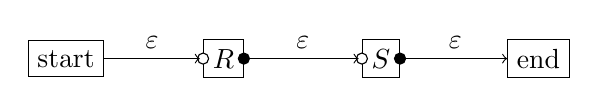
\begin{tikzpicture}[node distance=2cm]
      \node[draw] (A) at (0, 0) {start};
      \node[draw, right of=A] (R) {\(R\)};
      \draw[fill=white] (R.west) circle (2pt) node[inner sep=1pt] (R_start) {};
      \draw[fill=black] (R.east) circle (2pt) node[inner sep=1pt] (R_end) {};
      \node[draw, right of=R] (S) {\(S\)};
      \draw[fill=white] (S.west) circle (2pt) node[inner sep=1pt] (S_start) {};
      \draw[fill=black] (S.east) circle (2pt) node[inner sep=1pt] (S_end) {};
      \node[draw, right of=S] (B) {end};
      \draw[->] (A) -- node[above] {\(\varepsilon\)} (R_start);
      \draw[->] (R_end) -- node[above] {\(\varepsilon\)} (S_start);
      \draw[->] (S_end) -- node[above] {\(\varepsilon\)} (B);
    \end{tikzpicture}
    \caption{Concatenation \((RS)\)}\label{fig:enfa-1}
  \end{figure}
  \item if there's a union of regular expressions \(R\) and \(S\), then
    create NFA of type shown in figure \ref{fig:enfa-2})
  \begin{figure}[!htbp]
    \centering
    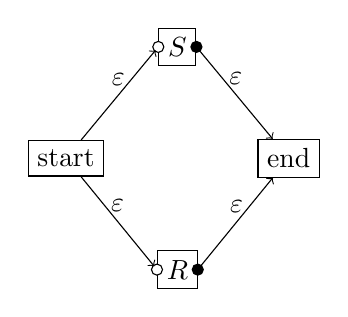
\begin{tikzpicture}[node distance=2cm]
      \node[draw] (A) at (0, 0) {start};
      \node[draw, below right of=A] (R) {\(R\)};
      \draw[fill=white] (R.west) circle (2pt) node[inner sep=1pt] (R_start) {};
      \draw[fill=black] (R.east) circle (2pt) node[inner sep=1pt] (R_end) {};
      \node[draw, above right of=A] (S) {\(S\)};
      \draw[fill=white] (S.west) circle (2pt) node[inner sep=1pt] (S_start) {};
      \draw[fill=black] (S.east) circle (2pt) node[inner sep=1pt] (S_end) {};
      \node[draw, below right of=S] (B) {end};
      \draw[->] (A) -- node[above] {\(\varepsilon\)}(R_start);
      \draw[->] (A) -- node[above] {\(\varepsilon\)}(S_start);
      \draw[->] (R_end) -- node[above] {\(\varepsilon\)}(B);
      \draw[->] (S_end) -- node[above] {\(\varepsilon\)}(B);
    \end{tikzpicture}
    \caption{Union \((R|S)\)}\label{fig:enfa-2}
  \end{figure}
  \item if there's a Kleene star operation applied to regular expression \(R\),
    then create NFA shown in figure \ref{fig:enfa-3}.
  \begin{figure}[!htbp]
    \centering
    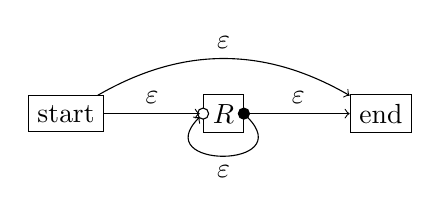
\begin{tikzpicture}[node distance=2cm]
      \node[draw] (A) at (0, 0) {start};
      \node[draw, right of=A] (R) {\(R\)};
      \node[draw, right of=R] (B) {end};
      \draw[fill=white] (R.west) circle (2pt) node[inner sep=1pt] (R_start) {};
      \draw[fill=black] (R.east) circle (2pt) node[inner sep=1pt] (R_end) {};

      \draw[->] (A) to[out=30, in=150] node[above]
        {\(\varepsilon\)}(B);
      \draw[->] (A) to node[above] {\(\varepsilon\)} (R_start);
      \draw[->] (R_end) to node[above] {\(\varepsilon\)} (B);
      \draw[->] (R_end) to[out=-45,in=-135, looseness=4] node[below] {\(\varepsilon\)}
        (R_start);
    \end{tikzpicture}
    \caption{Kleene star \((R^*)\)}\label{fig:enfa-3}
  \end{figure}

\end{enumerate}

\subsection{\(\varepsilon\)-NFA to NFA}

\begin{enumerate}
  \item Reduce ,,unnecessary'' \(\varepsilon\)-transitions (see figure
    \ref{fig:enfa-to-nfa-1})
  \begin{figure}[!htbp]
    \centering
    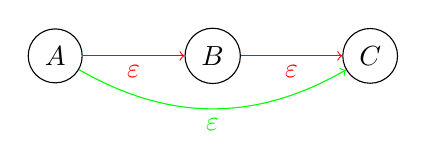
\begin{tikzpicture}[node distance=2cm]
      \node[draw, circle] (A) at (0, 0) {\(A\)};
      \node[draw, circle, right of=A] (B) {\(B\)};
      \node[draw, circle, right of=B] (C) {\(C\)};

      \draw[->, color=red] (A) to node[below] {\(\varepsilon\)} (B);
      \draw[->, color=red] (B) to node[below] {\(\varepsilon\)} (C);
      \draw[->, color=green] (A) to[out=-30, in=-150] node[below] {\(\varepsilon\)} (C);
    \end{tikzpicture}
    \caption{Removing ,,unnecessary'' \(\varepsilon\)-transitions}%
    \label{fig:enfa-to-nfa-1}
  \end{figure}
  \item Back-propagate terminating states over \(\varepsilon\)-transitions
    (see figure \ref{fig:enfa-to-nfa-2})
  \begin{figure}[!htbp]
    \centering
    \begin{tikzpicture}[node distance=2cm]
      \node[draw, circle] (A) at (0, 0) {\(A\)};
      \node[draw, circle, double, right of=A] (B) {\(B\)};
      \node[draw=none, right of=B, xshift=-0.5cm] (T_1) {};
      \node[draw=none, right of=T_1, xshift=-0.5cm] (T_2) {};

      \node[draw, circle, double, right of=T_2, xshift=-0.5cm] (A_1) {\(A\)};
      \node[draw, circle, double, right of=A_1] (B_1) {\(B\)};

      \draw[->] (A) to node[below] {\(\varepsilon\)} (B);
      \draw[-implies, double equal sign distance] (T_1) to (T_2);
      \draw[->] (A_1) to node[below] {\(\varepsilon\)} (B_1);
    \end{tikzpicture}
    \caption{Back-propagating terminating states over
    \(\varepsilon\)-transition}%
    \label{fig:enfa-to-nfa-2}
  \end{figure}
  \item Perform symbol-transition (see figure \ref{fig:enfa-to-nfa-3})
  \begin{figure}[!htbp]
    \centering
    \begin{tikzpicture}[node distance=2cm]
      \node[draw, circle] (A) at (0, 0) {\(A\)};
      \node[draw, circle, right of=A] (B) {\(B\)};
      \node[draw, circle, right of=B] (C) {\(C\)};
      \node[draw=none, right of=C, xshift=-0.5cm] (T_1) {};
      \node[draw=none, right of=T_1, xshift=-0.5cm] (T_2) {};

      \node[draw, circle, right of=T_2, xshift=-0.5cm] (A_1) {\(A\)};
      \node[draw, circle, right of=A_1] (B_1) {\(B\)};
      \node[draw, circle, right of=B_1] (C_1) {\(C\)};

      \draw[->] (A) to node[below] {\(\varepsilon\)} (B);
      \draw[->] (B) to node[below] {\(c\)} (C);

      \draw[-implies, double equal sign distance] (T_1) to (T_2);

      \draw[->] (A_1) to node[below] {\(\varepsilon\)} (B_1);
      \draw[->] (B_1) to node[below] {\(c\)} (C_1);
      \draw[->] (A_1) to[out=-45,in=-135] node[below] {\(c\)} (C_1);
    \end{tikzpicture}
    \caption{Performing symbol-transition}%
    \label{fig:enfa-to-nfa-3}
  \end{figure}
  \item Remove \(\varepsilon\)-transitions.
\end{enumerate}

\section{NFA to DFA}
%TODO


\section{Recurrence relations}

\begin{definition}[Recurrence relation]
  Recurrence relation is an equation
  that expresses each element of a sequence
  as a function of the preceding ones.
\end{definition}

\begin{example}
  \[
  \begin{cases}
    a_0 = 1 \\
    a_n = a_{n - 1} + n, & n \ge 1
  \end{cases}
  .\]
\end{example}

\begin{definition}[Characteristic equation]
  Informally, characteristic equation of a linear recurrence relation
  is recurrence relation equation
  where all elements of sequence \(a_i\) are replaced with \(r^i\).
\end{definition}

Characteristic equation can be used to obtain closed form of
a linear recurrence that doesn't contain \(n\) in equation.
It's very similar to linear ordinary differential equations.

\section{Asymptotic analysis}

Informally, asymptotic analysis is a method of describing how
a function behaves on infinity.

Functions \(f(x)\) and \(g(x)\) in relation \(f(x) \sim g(x)\)
if  \(\lim_{x \to \infty} \frac{f(x)}{g(x)} = 1\).
Functions \(f(x)\) and \(g(x)\) are \textit{asymptotically equivalent}.

\section{Divide-and-conquer algorithms analysis}

Divide and conquer algorithm is an algorithm
that recursively breaks down a problem into
2+ sub-problems, until they become simple enough
to be solved directly. Then,
the result of sub-problems is ,,merged'',
or ,,combined''.

For example, \textit{merge sort}
is a divide-and-conquer algorithm.
\[
  T(n) =
\begin{cases}
  \Theta(1) & \text{if}\ n = 1, \\
  T(\lfloor n/2 \rfloor) + T(\lceil n/2 \rceil) + \Theta(n) & \text{otherwise}
\end{cases}
.\]
Here \(\Theta(n)\) is the time complexity needed to merge two sorted subarrays
that were obtained by \(T(\lfloor n/2 \rfloor)\) and \(T(\lceil n/2 \rceil)\).

\begin{definition}[Master theorem]
  Master theorem provides an asymptotic analysis
  for recurrence relations of type
  \[
  T(n) = a T(n / b) + f(n)
  .\]
  Here \(a\) represents the number of sub-problems,
  and  \(b\) the ,,size'' of the sub-problem
  (\(a \in \mathbb{N}\), \(b > 0\)).
\end{definition}

\newcommand\ccrit{{c_\text{crit}}}

Let \(\ccrit = \log_b a\).
Then
\begin{enumerate}
  \item If \(f(n) \in O(n^c)\), where  \(c < \ccrit\), then
    work to split/recombine is dwarfed actual sub-problems.
    Therefore, \(T(n) \in \Theta(n^\ccrit)\).
  \item If \(f(n) \in \Omega(n^c)\), where \(c > \ccrit\)
    \textit{and}
    \(a f(n/b) \le k f(n)\) for some \(k < 1\),
    then
    work to split/recombine ,,outweighs'' actual sub-problems.
    Therefore, \(T(n) \in \Theta(f(n))\).
  \item If \(f(n) \in \Theta(n^\ccrit \log^k n)\), then
    the work to split/recombine is comparable to sub-problems.
    \begin{enumerate}
      \item \(k > -1\), then \(T(n) \in \Theta(n^\ccrit \log^{k + 1} n)\)
      \item \(k = -1\), then \(T(n) \in \Theta(n^\ccrit \log \log n)\)
      \item \(k < -1\), then \(T(n) \in \Theta(n^\ccrit)\)
    \end{enumerate}
\end{enumerate}

\begin{definition}[Akra--Bazzi method]
  Akra--Bazzi method provides an asymptotic analysis for recurrence
  relations of type
  \[
    T(n) = f(n) + \sum_{i = 1}^k a_i T(b_i n + h_i(n)),
  \]
  where
  \begin{enumerate}
    \item \(a_i \in \mathbb{N}\),
    \item \(0 < b_i < 1\),
    \item \(|h_i(n)| \in O(\frac{n}{\log^2 n})\),
    \item \(|f'(n)| \in O(n^c)\) for some \(c\).
  \end{enumerate}
  Then, \(p\) is such that \(\sum_{i = 1}^k a_i b_i^k = 1\).
  Then,
  \[
    T(n) \in \Theta
    \left( n^p \left( 1 + \int_1^n \frac{f(x)}{x^{p + 1}} \dd x \right)  \right)
  .\]
\end{definition}


\section{Generating function}

\begin{definition}[Formal power series]
  Formal power series \(f(x)\) is
  \[
    f(x) = \sum_{n = 0}^\infty a_n x^n
  \]
  where \(x\) is considered to be a \textit{variable}
  and \(a_n\) are elements of a sequence.
  It should not be treated as a function, rather
  it should be treated as an algebraic object.
\end{definition}
Algebraic operations (such as addition, subtraction, multiplication)
can be done on formal power series.
\begin{definition}[Generating function (GF)]
  A generating function for a sequence \(a_n\) is a
  formal power series for the sequence.
\end{definition}

\subsection{Solving linear recurrences using GF}

The idea is to express all \(a_i\) in linear recurrence using GF.
\begin{example}
  \(a_n = 2 a_{n - 1} + 2\),  \(a_0 = 1\).
  Let  \(G(x) = \sum_{i = 1}^\infty a_n x^n\).
  Then,
  \begin{align*}
    \sum_{i = 1}^\infty a_{n - 1} x^n &= x G(x) + a_0 x^1 = x G(X) + x \\
    \sum_{i = 1}^\infty 2 x^n &= \frac{2x}{1 - x}.
  \end{align*}
  Therefore,
  \[
    G(x) = 2 (x G(x) + x) + \frac{2x}{1 - x}
    \implies
    G(x)(1 - 2x) = 2x\frac{-x + 2}{1 - x}
    \implies
    G(x) = 2x \frac{-x + 2}{(1-x)(1-2x)}
  .\]
  Now apply partial fraction decomposition
  \[
  \frac{A}{1 - x} + \frac{B}{1 - 2x} = \frac{-x + 2}{(1-x)(1-2x)}
  \implies
  \frac{A(1 - 2x) + B(1-x)}{(1-x)(1-2x)} = \frac{-x + 2}{(1-x)(1-2x)}
  \implies
  \begin{cases}
    -2A - B = -1 \\
    A + B = 2
  \end{cases}
  .\]
  Therefore, \(A = -1\), \(B = 3\).
  \[
    G(x) = 2x \left( \frac{-1}{1 - x} + \frac{3}{1 - 2x} \right)
  .\]
  \begin{align*}
    \frac{1}{1 - 2x} &= \sum_{n = 0}^\infty 2^n x^n \\
    \frac{1}{1 - x} &= \sum_{n = 0}^\infty 1 \cdot x^n
  \end{align*}
  Therefore,
  \[
    G(x) = 2x \sum_{n = 0}^\infty (-1 + 3 \cdot 2^n) x^n
    = \sum_{n = 1}^\infty 2 (-1 + 3 \cdot 2^{n - 1}) x^n
  .\]
  Therefore,
  \[
    a_n = 2(-1 + 3 \cdot 2^{n - 1}) = -2 + 3 \cdot 2^n
  .\]
\end{example}

\subsection{Solving combinatorial problems using generating functions}

Basically, the generating functions can be used to solve combinatorial
problems if the task is about choosing something.

\begin{example}
  Find the number of integers solutions to equation
  \[
    a_1 + a_2 + \ldots + a_n = S, 0 \le a_i \le 9
  .\]
  The problem is equivalent to find coefficient of \(x^S\)
  in polynomial
   \[
     \underbrace{(x^0 + x^1 + \ldots + x^9) \ldots (x^0 + x^1 + \ldots +
     x^9)}_{n\ \text{times}} = (x^0  + x^1 + \ldots + x^9)^n
  .\]
  GF for sequence
  \[
    \begin{cases}
      a_n = 1 & 0 \le n \le 9 \\
      a_n = 0 & \text{otherwise}.
    \end{cases}
  \]
  is
  \[
    G(x) = \frac{1 - x^{10}}{1 - x}
  .\]
  Therefore, the task is to find coefficient of \(x^S\)
  in \(\left( \frac{1 - x^{10}}{1 - x} \right)^n \).
\end{example}

\newcommand\FBS{\boldsymbol{F}}
\begin{example}
  A \textit{Fibonacci composition} of \(n\) is a multiset \(\langle \FBS, m
  \rangle\) with underlying set of Fibonacci numbers \(\FBS\)
  such that \(\sum_{F \in \FBS} F \cdot m(F) = n\).
  The task is to find the number of Fibonacci compositions of \(n\).
  For example, \(n = 20\).
  Then, the task is to find coefficient of  \(x^{20}\) of
  \[
     \sum_{n = 1}^{\infty} (x + x^2 + x^3 + x^5 + x^8 + x^{13})^n
  \]
  \(n\) in sum represents the cardinality of multiset.
\end{example}



\section{Operators and annihilator}

\begin{definition}[Operator]
  Operator is higher-order function (i.e. that takes one or more functions and
  produces a function)
\end{definition}
Examples of operators:
\begin{enumerate}
  \item differential operator --- \(\frac{\dd}{\dd x}\)
  \item integral operator --- \(\int \dd x\)
  \item sum (takes two functions and returns their sum) ---
    \((f + g)(n) = f(n) + g(n)\)
  \item scale --- \((\alpha \cdot f)(n) = \alpha f(n)\)
\end{enumerate}
\newcommand\EE{\boldsymbol{E}}
\begin{definition}[Shift operator]
  Shift operator \(\EE\) is an operator with semantics:
   \[
    (\EE f)(n) = f(n + 1)
  .\]
\end{definition}
The sum, scale and shift operators are all linear.
\begin{definition}[Annihilator]
  An annihilator of a function \(f(n)\)
  is a non-trivial operator \(X\)
  such that \(Xf \equiv 0\).
\end{definition}
\begin{example}
  Given a function \(f(n) = \alpha a^n\) and operator  \(X = \EE - a\).
  Let's apply \(X\) to \(f(n)\):
   \[
     (\EE - a)f = \EE f(n) - a \cdot f(n) = f(n + 1) - a f(n)
     = \alpha a^{n + 1} - a \alpha a^n
     = a \alpha a^n - a \alpha a^n = 0
  .\]
  Therefore, \((\EE - a)\) is an annihilator for function  \(f(n) = \alpha a^n\).
\end{example}

\subsection{Solving linear recurrences using annihilators}

The idea is to consider \(f(n) = a_n\) and
apply operators to the recurrence equation so that it equals 0.
By the operators that were applied it's easy to find out
the form of the closed-formula.

\begin{example}
  \(a_n = 4 a_{n - 1} + 5 a_{n - 2}\), \(a_0 = 1\), \(a_1 = 17\).
  Note: \(\EE a_n = a_{n + 1}\).
  Therefore, \(\EE^2 a_{n - 2} = 4 \EE a_{n - 2} + 5 a_{n - 2}\).
  \[
    (\EE^2 - 4 \EE - 5) a_{n - 2} = 0
    \iff
    (\EE + 1)(\EE - 5) a_{n - 2} = 0
  .\]
  It's known that \(\EE - 5\) annihilates \(\alpha 5^n\),
  and \(\EE + 1\) annihilates \(\beta (-1)^n\).
  Therefore, the ,,shape'' of the \(a_n\) is
   \[
    a_n = \alpha 5^n + \beta (-1)^n
  .\]
  To find \(\alpha\) and \(\beta\) use \(a_0\) and \(a_1\)
  \[
  \begin{cases}
    a_0 = \alpha 5^0 + \beta (-1)^0 = \alpha + \beta = 1 \\
    a_1 = \alpha 5^1 + \beta (-1)^1 = 5 \alpha - \beta = 17
  \end{cases}
  \implies
  \begin{cases}
    \alpha = 3 \\
    \beta = -2
  \end{cases}
  .\]
  Therefore, the answer is
  \[
  a_n = 3 \cdot 5^n - 2 \cdot (-1)^n
  .\]
\end{example}
\begin{example}
  \(a_n = 4 a_{n - 1} - 4 a_{n - 2}\), \(a_0 = 3\), \(a_1 = 11\).
  \[
    \EE^2 a_{n - 2} = 4 \EE a_{n - 2} - 4 a_{n - 2}
    \implies
    (\EE^2 - 4 \EE + 4) a_{n - 2} = 0
    \implies
    (\EE - 2)^2 a_{n - 2} = 0
  .\]
  It's not hard to prove that \((\EE - a)^2\) annihilates
  \((\alpha n + \beta) a^n\).
  Therefore,
  \[
  a_n = (\alpha n + \beta) 2^n
  .\]
  \[
  \begin{cases}
    a_0 = (\alpha \cdot 0 + \beta) 2^0 = \beta = 3 \\
    a_1 = (\alpha \cdot 1 + \beta) 2^1 = 2 (\alpha + \beta) = 11
  \end{cases}
  \implies
  \begin{cases}
    \alpha = 5/2 \\
    \beta = 3
  \end{cases}
  .\]
  \[
    a_n = (2.5 n + 3) 2^n
  .\]
\end{example}
\end{document}
